\documentclass[11pt,english]{article}

\setlength{\oddsidemargin}{0cm}
\setlength{\topmargin}{-2cm}
\setlength{\textwidth}{160mm}
\setlength{\textheight}{230mm}

\usepackage[english]{babel}                      
\usepackage[utf8]{inputenc}                    
\usepackage{amsmath}                             
\usepackage{amssymb}                               
\usepackage[pdftex]{graphicx}                    
\usepackage{float} 
\usepackage{subfigure} 
\usepackage[ruled,linesnumbered]{algorithm2e}
\usepackage[colorlinks, linkcolor=blue]{hyperref}
\usepackage{appendix}

\newtheorem{lemma}{Lemma}

\DeclareGraphicsExtensions{.jpg,.mps,.pdf,.png}    

\begin{document}

\title
{
    \textbf{Project CPA \\ Minimum enclosing circle problems\\}
}

\author
{
    \\
    \\
    Submitted by
    \\
    \\
    \\
    \\
    \textbf{Haotian Xue}
    \\
    \textbf{Hejun Cao}
    \\
    M2 Science et Technologie du Logiciel 2024-2025
    \\
    Sorbonne Universite (SU UPMC)
    \\
    \\
    \\
    Under the guidance of 
    \\
    \\
    \textbf{\href{https://www-npa.lip6.fr/~buixuan/}{\textcolor{black}{Binh-Minh Bui-Xuan}}}
    \\
    Laboratoire d'Informatique de Paris 6 (LIP6)
    \\
    Centre National de la Recherche Scientifique (CNRS)
    \\
    Sorbonne Universite (SU UPMC)
}

\date{05/10/2024}

\maketitle

\begin{figure}[htbp]
    \begin{center}
        
\includegraphics[height=3cm]{./src/logo_lip6.png}
    \end{center}
\end{figure}

\begin{figure}[htbp]
    \begin{center}
        
\includegraphics[height=3cm]{./src/Science_Sorbonne_logo.png}
    \end{center}
\end{figure}

\pagebreak

\tableofcontents

\pagebreak

\section{Introduction}

\indent 

Le projet que nous entreprenons vise à créer un clone du célèbre outil egrep utilisé dans les systèmes Unix pour la recherche de motifs dans des fichiers texte. L'objectif principal de ce projet est de concevoir une version offline et desktop de ce moteur de recherche, en se limitant à certaines conventions de la norme ERE (Expressions Régulières Étendues). Les éléments de base que nous allons prendre en compte sont : les parenthèses (), l'alternative |, la concaténation (implicite), l'opération étoile *, le point (caractère universel .), ainsi que les lettres ASCII.

\indent L'enjeu de ce projet est double : non seulement il permet de se familiariser avec des concepts algorithmiques fondamentaux liés à la recherche de motifs, mais il met également en pratique des structures de données efficaces comme les automates finis déterministes (DFA) et non déterministes (NFA), ainsi que l'algorithme de recherche de motifs de Knuth-Morris-Pratt (KMP). Chacune de ces approches présente des avantages et des inconvénients spécifiques selon les contextes d'utilisation, que ce projet permet d'explorer.

\indent L'un des aspects les plus complexes de ce projet réside dans la conversion des expressions régulières en automates finis, notamment en NFA, puis en DFA, permettant ainsi un traitement plus rapide des recherches. De plus, nous implémentons une recherche par KMP pour les cas où les motifs sont des chaînes simples. L'objectif final est de fournir un moteur de recherche performant et fonctionnel capable de traiter efficacement de grands volumes de texte, tout en respectant les contraintes de performance et de simplicité imposées par une application desktop.

\indent La phase de test et d'évaluation des performances est cruciale dans ce projet. En effet, nous utiliserons la base de données Gutenberg, qui propose de nombreux textes disponibles en libre accès, pour tester nos algorithmes sur des corpus variés et de grande taille. Ces tests nous permettront d'analyser les performances de nos implémentations et d'identifier les points d'amélioration possibles.

\section{Problème Défini}

\indent

Le projet consiste à concevoir un moteur de recherche offline capable de reproduire le comportement de la commande egrep. Plus précisément, le moteur doit permettre la recherche de motifs complexes au sein de fichiers texte en utilisant des expressions régulières. Cependant, contrairement à un support complet des expressions régulières, notre implémentation se limite à un sous-ensemble des fonctionnalités de la norme ERE (Expressions Régulières Étendues).

\indent L'objectif du projet est donc de proposer une solution qui convertit les expressions régulières décrites ci-dessus en une structure efficace, capable de trouver rapidement les occurrences de motifs dans de grands fichiers texte. L'accent est mis sur la performance du moteur de recherche, ainsi que sur la capacité à traiter efficacement les expressions régulières grâce à des techniques avancées comme les automates finis et l'algorithme KMP.

\indent Cependant, en raison de la nature même de l'algorithme KMP, nous ne pouvons rechercher que le texte donné au lieu de faire correspondre une expression régulière complète.

\section{Structure de Données}

\subsection{NFA et NFAState}

\indent 

Classe NFA contient les états de départ et de fin de l'automate.


\indent Pour classe NFAState, chaque état d'un NFA est représenté par un objet qui stocke un ensemble de transitions vers d'autres états en fonction de caractères ou d'$\varepsilon $-transitions.

\subsection{DFA et DFAState}

\indent

Classe DFA est responsable de la conversion du NFA en DFA, ainsi que de la recherche dans le texte.

\indent Pour classe DFAState, chaque état du DFA possède des transitions déterministes basées sur un seul caractère et indique si l'état est un état acceptant (fin de motif).



\section{Aho-Ullman}

\indent

L'algorithme de conversion NFA en DFA, tel que décrit par Aho et Ullman dans leur ouvrage, constitue l'un des piliers fondamentaux de notre projet. Cet algorithme est crucial pour optimiser la recherche de motifs complexes dans les fichiers texte en transformant des expressions régulières en automates. Nous détaillerons ici les principales étapes de l'algorithme et analyserons la complexité temporelle de chaque étape, ainsi que son comportement dans les cas optimaux et pessimistes.

\subsection{Conversion d'une expression régulière en NFA}

L'algorithme commence par la conversion d'une expression régulière en un automate fini non déterministe (NFA). Cette étape est relativement simple et suit des règles déterministes :

- Chaque caractère ou élément de l'expression régulière (comme `a`, `b`, etc.) est représenté par un état du NFA.
- Les opérateurs réguliers comme l'alternance (`|`), l'étoile (`*`), et la concaténation sont gérés en ajoutant de nouveaux états et transitions au NFA. Par exemple :
    - L'opérateur `|` crée deux chemins parallèles à partir d'un même état initial.
    - L'opérateur `*` permet de retourner à un état précédent ou d'avancer sans lire de caractère.
    - La concaténation relie deux états de manière séquentielle.
  
La complexité de cette phase est proportionnelle à la taille de l'expression régulière, soit \textbf{O(k)}, où $k$ est la longueur de l'expression régulière. À ce stade, le nombre d'états est contrôlé et reste relativement petit, car les NFA gèrent plusieurs transitions depuis un même état.

\subsection{Conversion du NFA en DFA}

La partie la plus coûteuse de l'algorithme est la conversion du NFA en un DFA à l'aide de l'algorithme de construction de sous-ensembles. Chaque état du DFA représente un ensemble d'états du NFA, et la transition d'un état à un autre dans le DFA correspond à des transitions multiples dans le NFA.

Cette phase suit les étapes suivantes :
- **Fermeture epsilon** : Pour chaque état du NFA, on calcule la fermeture epsilon (`ε-closure`), c'est-à-dire l'ensemble des états accessibles sans lire de caractère (via des transitions epsilon). Cela permet de définir des états déterministes dans le DFA.
- **Détermination des transitions** : Pour chaque symbole de l'alphabet, on calcule les transitions possibles à partir des états actuels du NFA et on les regroupe pour former un état unique dans le DFA.
- **Ajout des états et transitions au DFA** : Si un nouvel ensemble d'états est trouvé (un ensemble non encore exploré), il est ajouté au DFA avec les transitions correspondantes.

La complexité de cette conversion dépend du nombre d'états du NFA. Dans le pire des cas, un NFA avec $n$ états peut générer un DFA avec jusqu'à $2^n$ états, ce qui correspond à une complexité exponentielle \textbf{O(2$^n$)}. Cependant, dans de nombreux cas pratiques, la taille réelle du DFA est bien inférieure à cette limite théorique, car beaucoup d'états potentiels ne sont jamais générés ou explorés.

\begin{algorithm}[htbp]
    \SetAlFnt{\footnotesize\sf}
    \SetKwInOut{Input}{inputs}
    \SetKwInOut{Output}{outputs}
    \SetAlgoProcName{Nom}{ConvertNFAtoDFA}

    \caption{ConvertNFAtoDFA}
    
    \Input{ $NFA$, $StartState$ }
    \Output{ DFA correspondant au $NFA$ }
    \Begin
    {
        DFAState $\leftarrow$ EpsilonClosure(StartState) \\
        Init DFA avec DFAState comme état de départ \\
        
        \While{DFAState non exploré}
        {
            \ForEach{symbole du NFA}
            {
                NextStates $\leftarrow$ Move(DFAState, symbole) \\
                DFAState' $\leftarrow$ EpsilonClosure(NextStates) \\
                
                \If{DFAState' n'existe pas}
                {
                    Ajouter DFAState' au DFA \\
                }
                Ajouter transition de DFAState vers DFAState' sur symbole \\
            }
        }
    }
\end{algorithm}

\subsection{Recherche dans le texte avec le DFA}

Une fois le DFA construit, la recherche dans le texte devient très efficace. Le DFA permet de traiter chaque caractère du texte en temps constant, car chaque état du DFA a une transition unique pour chaque symbole de l'alphabet.

Ainsi, la recherche de motifs dans un texte de longueur $m$ prend un temps linéaire, soit \textbf{O(m)}. Comme le DFA ne nécessite pas de revenir en arrière ou de considérer plusieurs chemins possibles, chaque caractère est traité une seule fois. Cela fait de l'approche DFA une méthode extrêmement rapide pour la recherche une fois que l'automate est construit.

\subsection{Analyse des Cas Optimaux et Pessimistes}

\textbf{Cas optimal :}

Dans le cas optimal, l'expression régulière est relativement simple, sans utilisation excessive d'opérateurs comme `|` ou `*`. Par exemple, une expression régulière comme `abc` ou même `a*b` génère un NFA avec peu d'états, et la conversion en DFA est rapide. Dans ce scénario, la complexité temporelle est linéaire par rapport à la taille de l'expression régulière, soit \textbf{O(k)} pour la construction du NFA et \textbf{O(m)} pour la recherche dans le texte. La taille du DFA reste petite, et la recherche est réalisée en temps linéaire.

Le cas optimal se produit donc lorsque l'expression régulière ne génère pas un grand nombre d'états dans le NFA, et lorsque les transitions entre les états sont simples.

\textbf{Cas pessimiste :}

Dans le pire des cas, l'expression régulière contient de nombreux opérateurs `|`, `*`, et des parenthèses imbriquées, ce qui entraîne une explosion du nombre d'états dans le NFA. Par exemple, une expression comme `(a|b|c)*` génère un nombre important de combinaisons d'états dans le NFA, et la conversion en DFA peut entraîner une explosion exponentielle du nombre d'états.

Dans ce cas, la complexité de la conversion NFA en DFA devient \textbf{O(2$^n$)}, où $n$ est le nombre d'états du NFA. Cela peut entraîner des temps de calcul très longs et une utilisation excessive de la mémoire. Cependant, une fois le DFA construit, la recherche dans le texte reste rapide, avec une complexité linéaire \textbf{O(m)}.

Le cas pessimiste survient lorsque l'expression régulière est très complexe, impliquant de nombreuses alternatives et répétitions, ce qui fait croître de manière exponentielle la taille du DFA.

\subsection{Conclusion pour Aho-Ullman}

L'algorithme de conversion NFA en DFA, bien que potentiellement coûteux en temps et en espace dans le pire des cas, reste une méthode extrêmement efficace pour la recherche de motifs complexes une fois le DFA construit. Le DFA permet une recherche en temps constant pour chaque caractère du texte, rendant cette approche particulièrement adaptée aux recherches répétées dans de grands fichiers texte. Cependant, dans le cas où l'expression régulière est extrêmement complexe, il est important de prendre en compte les limites de cet algorithme en termes de mémoire et de temps de conversion.


\section{KMP}

\indent

L'algorithme Knuth-Morris-Pratt (KMP) est un algorithme classique pour la recherche de motifs dans une chaîne de caractères. Il résout efficacement le problème de recherche en évitant les comparaisons redondantes, en utilisant une pré-analyse du motif pour construire un tableau de préfixes, appelé LTS ("longest proper prefix which is also a suffix").

\indent L'algorithme KMP fonctionne en deux phases :

\begin{itemize}
    \item [$\bullet$] Pré-traitement
    \\
    On calcule un tableau LTS qui, pour chaque position dans le motif, indique le plus long préfixe du motif qui est aussi un suffixe. Cela permet de déterminer où reprendre la recherche lorsqu'une comparaison échoue.
    
    \item [$\bullet$] Recherche
    \\
    Pendant la recherche dans le texte, lorsque le motif ne correspond pas au texte à une certaine position, le tableau LTS est utilisé pour savoir combien de caractères on peut sauter dans le texte sans re-vérifier des comparaisons inutiles.
\end{itemize}

\subsection{LTS et CarryOver}

\indent 

La recherche KMP que nous avons apprise en classe est en fait une version modifiée de l'approche de M. Binh-Minh Bui-Xuan. Nous calculons d'abord le tableau LTS traditionnel, puis le tableau CarryOver basé sur le tableau LTS, ce qui réduit le nombre de comparaisons sous les bandes frontières ainsi que les calculs répétés et les retours en arrière inutiles, en particulier lorsqu'il s'agit de faire correspondre un grand nombre de textes dupliqués.

\indent Prenons l'exemple de \textbf{P = mami}.

\indent Nous commençons par construire un tableau LTS, dont la première valeur est fixée à -1 et la seconde à 0, comme nous l'a enseigné notre professeur.
Ensuite, la troisième valeur est 0, car a et m ne sont pas identiques.
Ensuite, la quatrième valeur est 1, car "mam" constitue un préfixe et un sufixe, et le nombre de lettres identiques est 1.
La dernière valeur est 0, car "mami" ne constitue pas un préfixe et un suffixe.

\indent Le tableau \textbf{LTS} est donc \textbf{[-1, 0, 0, 1, 0]} 

\indent La complexité temporelle de cet partie est \textbf{O(M)} et M est la longueur des caractères à faire correspondre.
En effet, nous n'effectuons qu'une seule opération en boucle sur la chaîne de caractères.

\indent Nous construisons ensuite le tableau CarryOver.

\indent En classe, le professeur avait donné la formule suivante :

\begin{itemize}
    \item [$\bullet$] $\forall$i$\in$[0,n-1], si P[i] = P[LTS[i]] et LTS[LTS[i]] = -1, alors LTS[i] = -1 
    \item [$\bullet$] $\forall$i$\in$[0,n-1], si P[i] = P[LTS[i]] et LTS[LTS[i]] $\neq$ -1, alors LTS[i] = LTS[LTS[i]]
\end{itemize}

\indent Sur la base de ces deux formules, nous pouvons déterminer que le tableau \textbf{CarryOver} est \textbf{[-1, 0, -1, 0, 1]}.

\indent La complexité temporelle de cette partie est également \textbf{O(M)}, puisque nous n'effectuons toujours qu'une seule boucle.

\indent Par conséquent, la complexité temporelle totale de cette partie du calcul du tableau LTS et du tableau CarryOver est \textbf{O(M)}.

\subsection{Recherche}

\indent 

Nous commençons par initialiser deux indices i et j, i étant utilisé pour marquer la position du texte tandis que j est utilisé pour marquer la position de P .
Nous parcourons ensuite l'ensemble du texte et les quatre correspondances suivantes se produisent :

\begin{itemize}
    \item [$\bullet$] P[j] = Texte[i]
    \\
    Cela signifie que la lettre à la position actuelle du texte est la même que la lettre à la position correspondante de P. Nous devons ajouter 1 à chacun des indices i et j.
    \item [$\bullet$] j = -1
    \\
    Les valeurs négatives ne peuvent provenir que du tableau CarryOver. La présence de -1 signifie que la correspondance a échoué, auquel cas nous avançons i plus un jusqu'à la lettre suivante du texte et remettons j à 0.
    \item [$\bullet$] j $\neq$ -1 et P[j] $\neq$ Texte[i]
    \\
    Ce cas signifie que le texte ne correspond pas et que nous devons effectuer un saut de correspondance correspondant sur la base du tableau CarryOver au lieu de simplement reléguer j à 0. C'est ce qui rend l'algorithme KMP si efficace. Je mets ici j à CarryOver[j].
    \item [$\bullet$] j = M
    \\
    Cela signifie que nous avons terminé un match. Il suffit de sortir le contenu de la ligne où se trouve le texte, puis de mettre j à 0 et break. 

\end{itemize}

\indent L'algorithme de cette partie est mis en œuvre comme suit :

\begin{algorithm}[htbp]
    \SetAlFnt{\footnotesize\sf}
    \SetKwInOut{Input}{inputs}
    \SetKwInOut{Output}{outputs}
    \SetAlgoProcName{Nom}{KMPSearch}

    \caption{KMPSearch}
    
    \Input{ $Text$, $P$, $LineNum$  }
    \Output{ Le texte $Res$ contenant P et le nombre $Num$ de lignes qu'il contient  }
    \Begin
    {
        computeLTS

        computeCarryOver

        j $\leftarrow$ 0; i $\leftarrow$ 0

        \While{i $<$ N}
        {
            \If{j = -1 $||$ Text[i]=P[j]}
            {
               i++; j++
            }
            \Else
            {
               j $\leftarrow$ CarryOver[j]
            }  

            \If{j = M}
            {
                Print(LineNumber et Text a ce ligne)
                
                j $\leftarrow$ 0

                break;
            }
        }

    }
\end{algorithm}

\pagebreak

\indent La complexité temporelle de cette partie est O(N), où N est le nombre de caractères contenus dans le texte. Parce que nous n’avons parcouru le texte qu’une seule fois.

\subsection{Complexité temporelle}

\indent 

La complexité temporelle de l'ensemble de l'algorithme KMP est O(M+N). J'ai déjà analysé la complexité temporelle de chaque partie.

\section{Comparaison des performances}

\indent

Les conditions de l'équipement utilisé pour les tests étaient les suivantes :

\begin{itemize}
    \item [$\bullet$]   cpu     :   Intel i7 13650H
    \item [$\bullet$]   Ubuntu  :   24.04
    \item [$\bullet$]   RAM     :   16G 4800MHz
    \item [$\bullet$]   Java    :   Java 17
\end{itemize}

\subsection{Comparaison avec Mot}

\indent

Nous avons comparé les deux scénarios.
Dans le premier cas, nous avons cherché des mots sans possibilité de bifurcation, comme "Sargon".

\begin{figure}[htbp]
    \begin{center}
        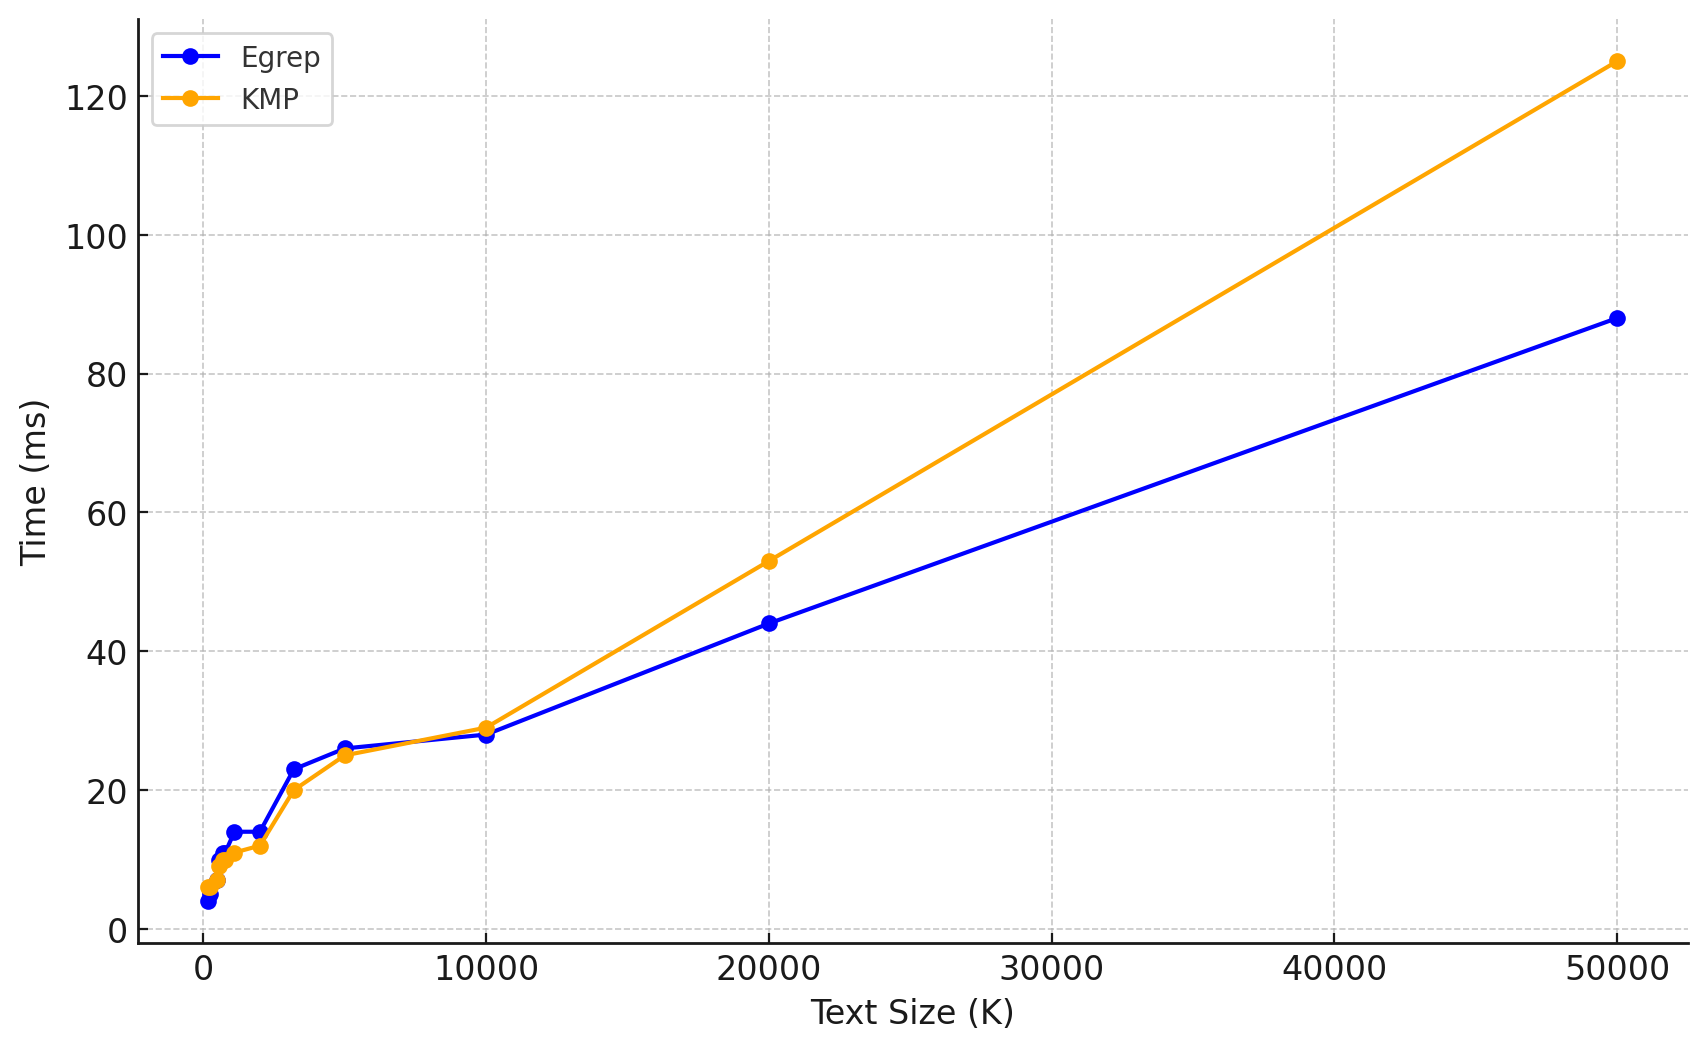
\includegraphics[height=7cm]{./src/Compare1.png}
    \end{center}
\end{figure}

\pagebreak

\subsection{Comparaison Regex et Mot}

\indent 

Par ailleurs, Egrep effectue une recherche à l'aide de l'expression régulière "S(a$|$r$|$g)+on", alors que KMP, en raison de limitations algorithmiques, recherche toujours “Sargon”.

\begin{figure}[htbp]
    \begin{center}
        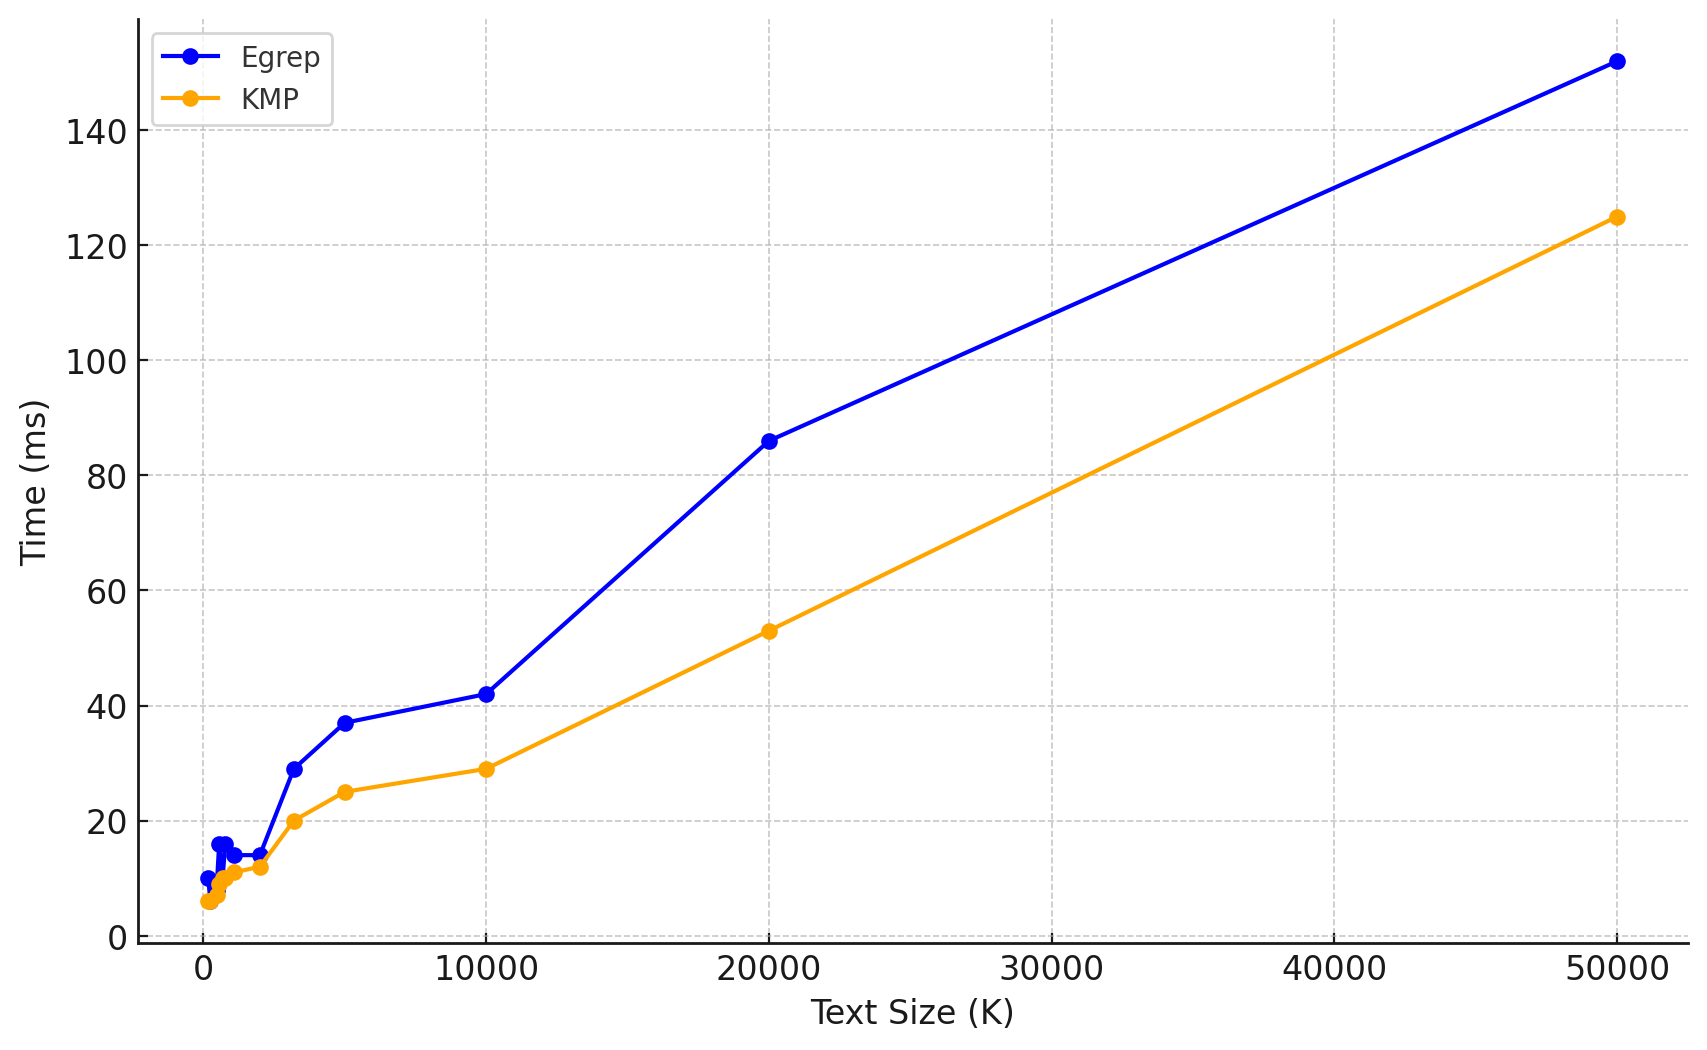
\includegraphics[height=7cm]{./src/Compare2.png}
    \end{center}
\end{figure}



\section{Optimisation}

\indent

Nous avons procédé à quelques optimisations de l'algorithme KMP. Normalement, l'algorithme KMP doit lire le texte ligne par ligne avant d'effectuer la recherche. Après l'optimisation, nous utiliserons plusieurs threads pour effectuer la recherche. Voici une comparaison du nombre de threads et du temps passé, pour un texte de 50M.

\begin{figure}[htbp]
    \begin{center}
        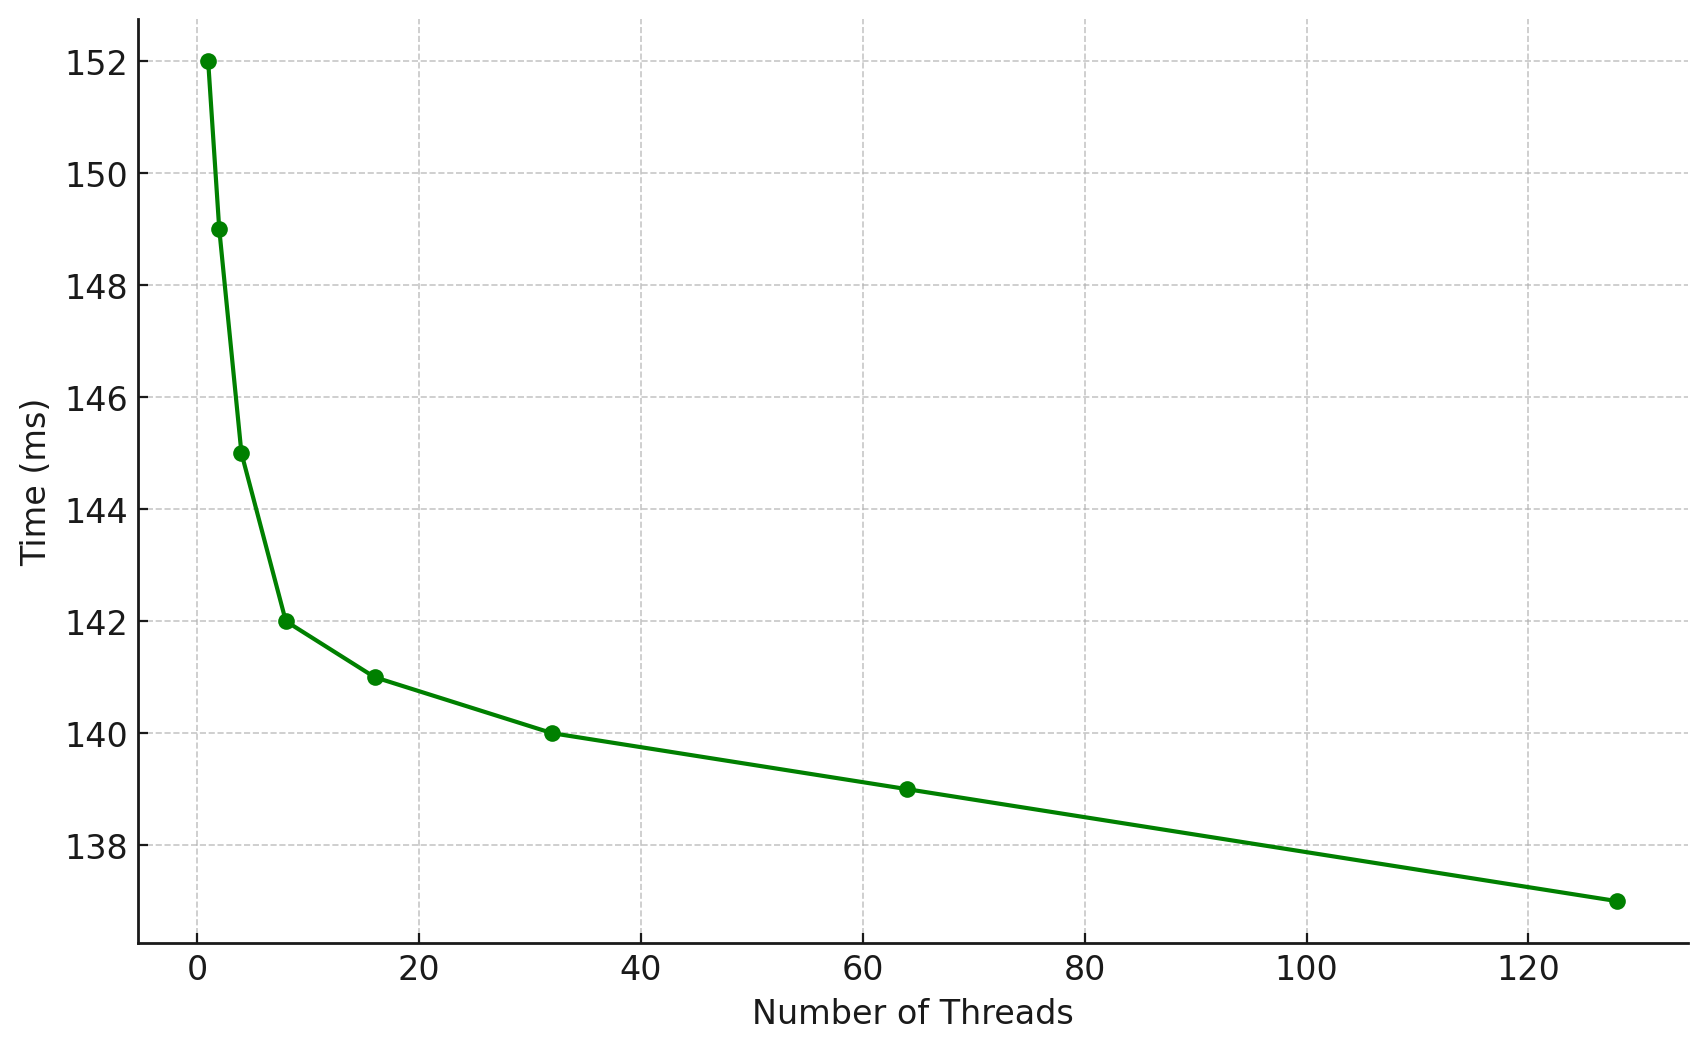
\includegraphics[height=7cm]{./src/Compare3.png}
    \end{center}
\end{figure}

\pagebreak

\indent On peut constater que le multithreading a un certain degré d'effet d'optimisation sur l'utilisation de l'algorithme KMP, mais il n'est pas évident, car le multithreading ne modifie pas la complexité temporelle de l'algorithme, mais accélère seulement la traversée du texte dans une certaine mesure.

\section{Conclusion}

\indent

D'après le tableau comparatif, nous pouvons constater que lors de l'utilisation de mots fixes tels que « Sargon », l'algorithme Egrep rencontrera son cas optimal, dans lequel les algorithmes Egrep et KMP ont la même complexité temporelle O(M+N). Dans ce cas, Egrep et KMP ont la même complexité en temps de O(M+N). Une fois qu'Egrep correspond à des expressions régulières relativement complexes, sa complexité en temps dans le pire des cas sera de O(2$^{n}$). En raison de la limitation de la taille du texte, le graphique linéaire ne peut pas bien montrer la courbe de changement.

\indent En ce qui concerne l'optimisation, nous n'avons pas trouvé de bonne solution d'optimisation algorithmique, nous avons donc choisi d'utiliser le multithreading, ce qui était aussi un bon moyen de réviser ce que nous avons appris l'année dernière.

\indent En résumé, le projet a mis en œuvre deux algorithmes classiques de recherche de motifs tout en explorant leurs forces et leurs limites dans différentes situations. Nous avons atteint l'objectif initial du projet en proposant un clone performant d'egrep, tout en explorant la solution algorithmique KMP et son optimisation.

\end{document}